\documentclass[aspectratio=169]{beamer}
\usetheme{Madrid}
\usepackage{graphicx}
\usepackage[utf8]{inputenc}
\usepackage{hyperref}
\usepackage{listings}
\usepackage{algorithm2e}


\begin{document}

\title{Introduction to neural networks}  
\subtitle{Simple neural network} 
\author[J.I. Vasquez]{\textbf{Juan Irving Vásquez} \\jivg.org}
\date{\today \copyright}
\institute[jivg.org]{Centro de Innovación y Desarrollo Tecnológico en Cómputo \\ Instituto Politécnico Nacional}
% logo of my university
\titlegraphic{
\includegraphics[height=1.2cm]{ipn-cidetec.png}\hspace{0.1cm}
\includegraphics[height=1.2cm]{escudoESCOM}}
\frame{\titlepage} 


\frame{
	\frametitle{Contents}
	\tableofcontents
}


\AtBeginSection[] { \begin{frame} \frametitle{Roadmap} \tableofcontents[currentsection] \end{frame} }

%%%%%%%%%%%%%%%%%%%%%%%%%%%%%%%%%%%%%%%%%%%%%%%%%%%%%%%%


\section{Modern Artificial Neuron}

\begin{frame}
	\frametitle{The big picture \footnote{https://medium.com/@lmpo/a-brief-history-of-ai-with-deep-learning-26f7948bc87b}}
	\centering
	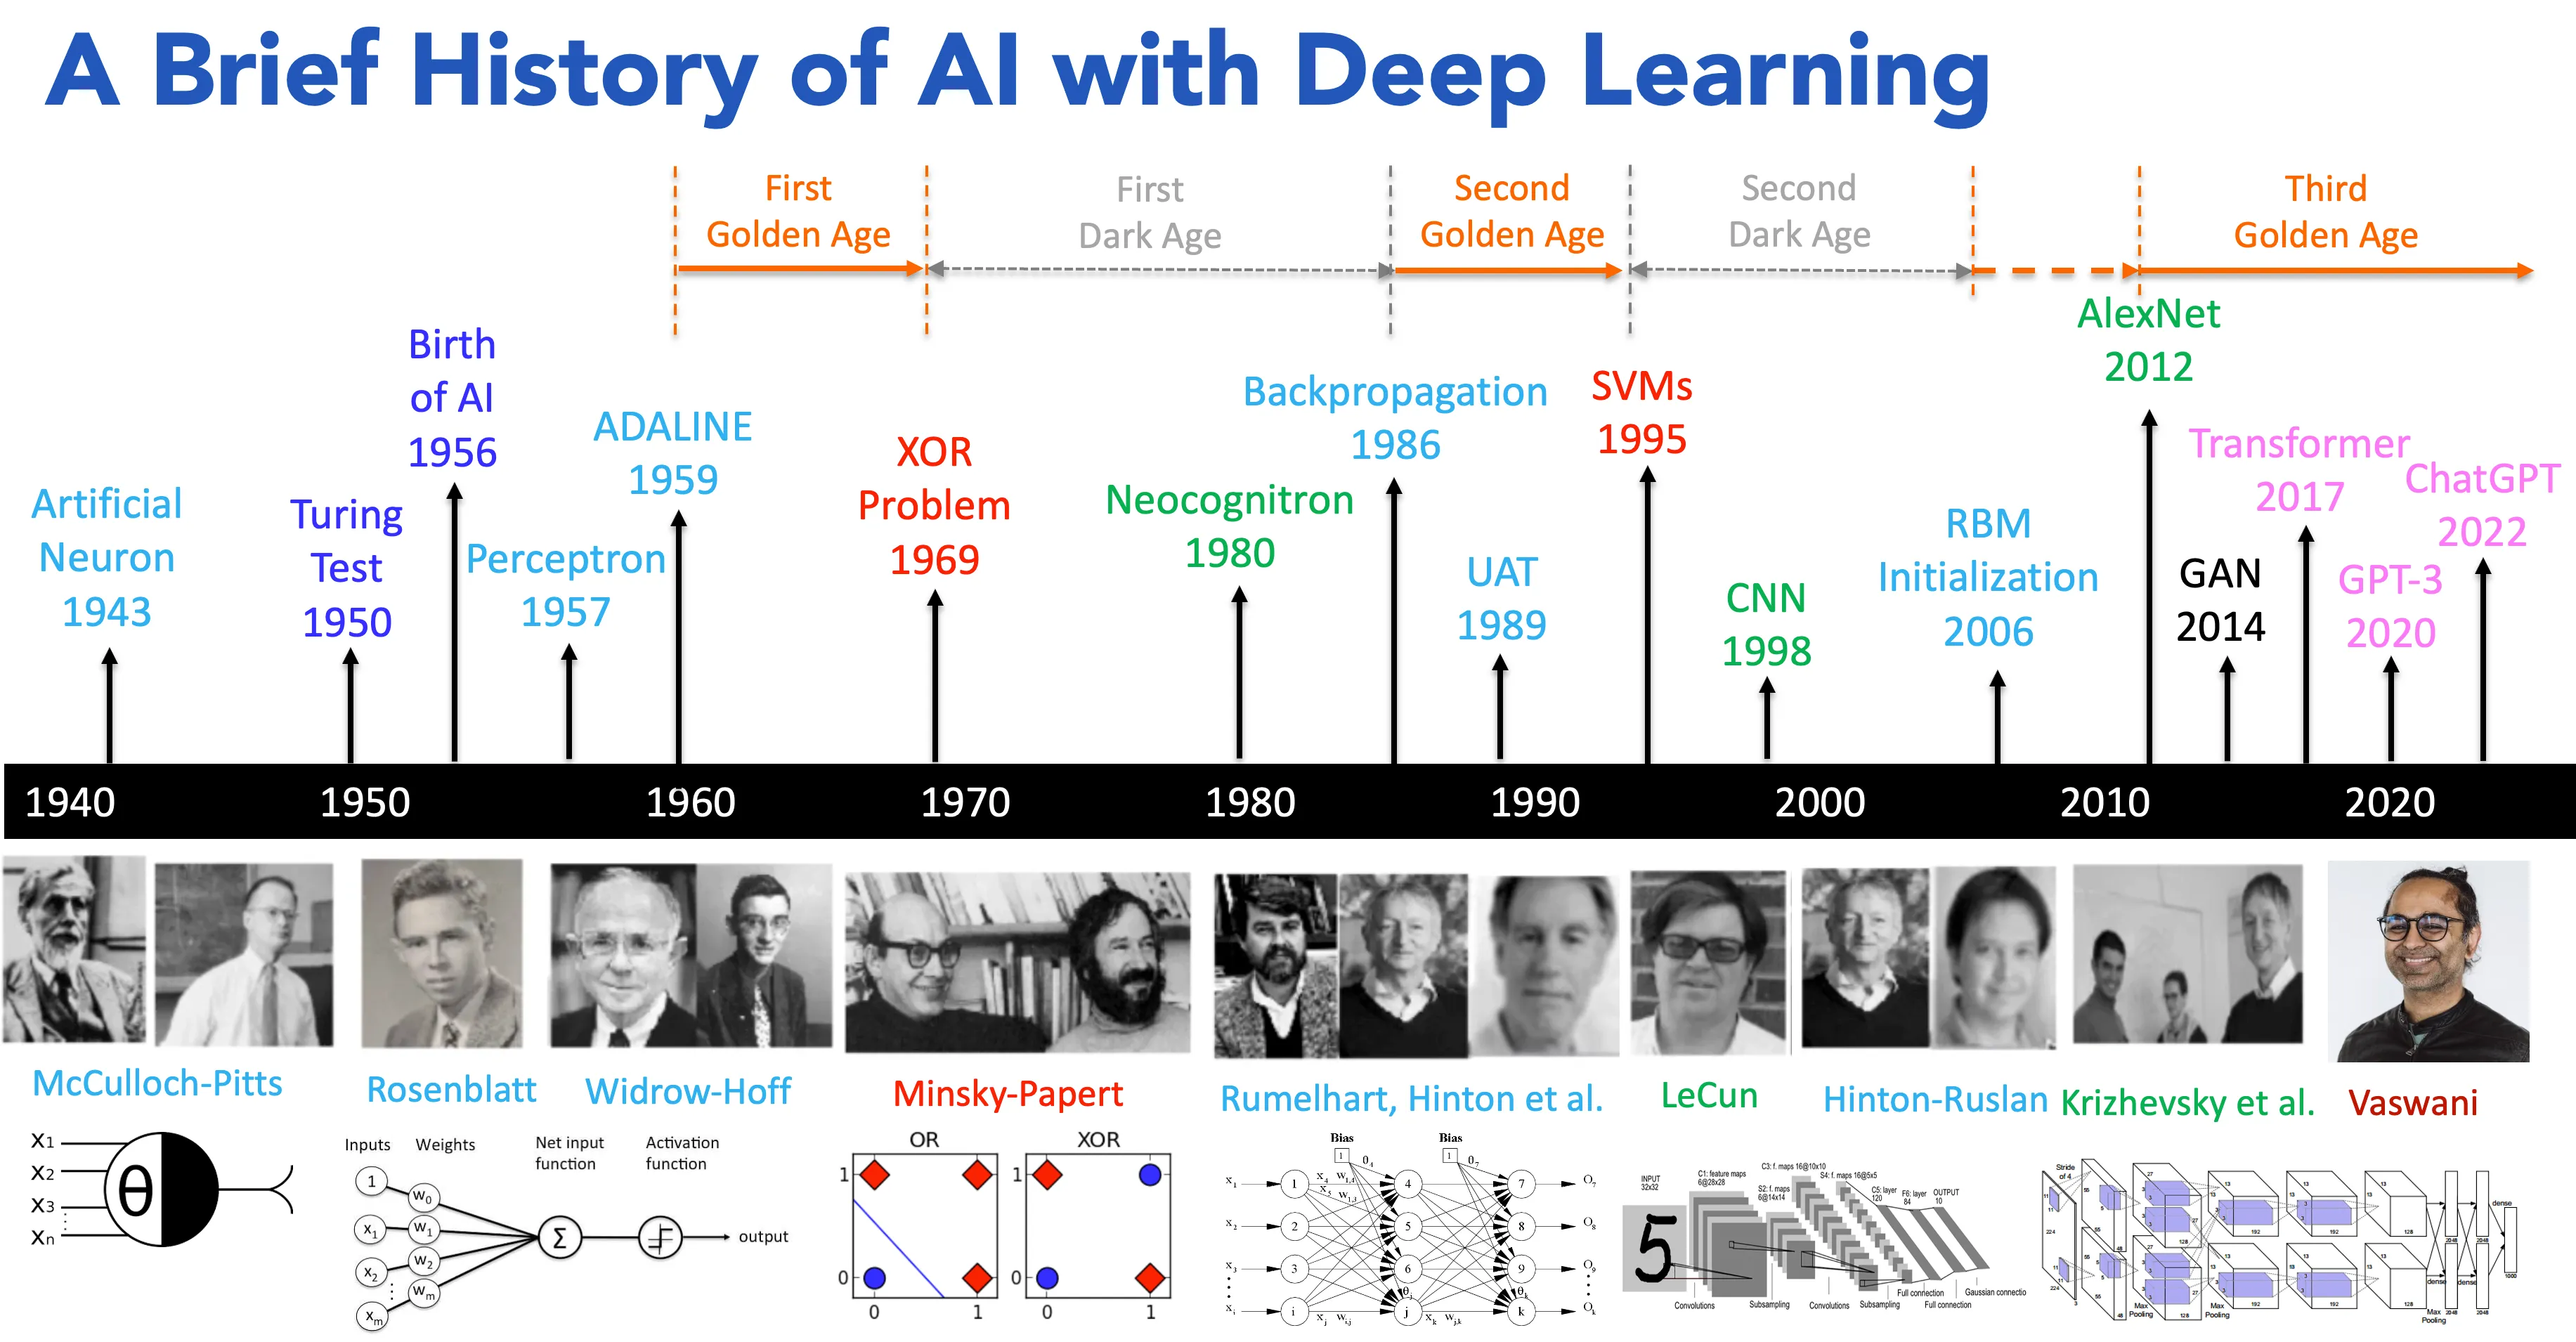
\includegraphics[trim={0 0 0 190},clip,width=0.92\textwidth]{timeline}
\end{frame}


\begin{frame}{Evolution: Rosenblatt Perceptron vs. Modern Neuron}
	
	\textbf{The Rosenblatt Perceptron}
	\begin{itemize}
		\item \textbf{Heaviside Step Function:} Output is strictly binary $y \in \{0, 1\}$.
		\item \textbf{Learning Rule:} Based on a simple heuristic error correction: $\Delta w = \eta (y - \hat{y})x$.
		\item \textbf{Mathematical Limitation:} The derivative is zero almost everywhere, making it non-differentiable.
	\end{itemize}
	
	\hrulefill
	
	\textbf{The Modern Neuron}
	\begin{itemize}
		\item \textbf{Continuous Activation:} Functions like Sigmoid or Tanh provide a smooth, differentiable mapping.
		\item \textbf{Error Surface:} Creates a continuous "loss landscape" that can be navigated.
		\item \textbf{Gradient Descent:} Enables optimization by iterative methods.
%		\[ w_{t+1} = w_t - \eta \nabla L(w_t) \]
	\end{itemize}
\end{frame}



\begin{frame}
	\frametitle{Modern Artificial Neuron}
	%\framesubtitle{One layer network}
	\begin{figure}
		\centering
		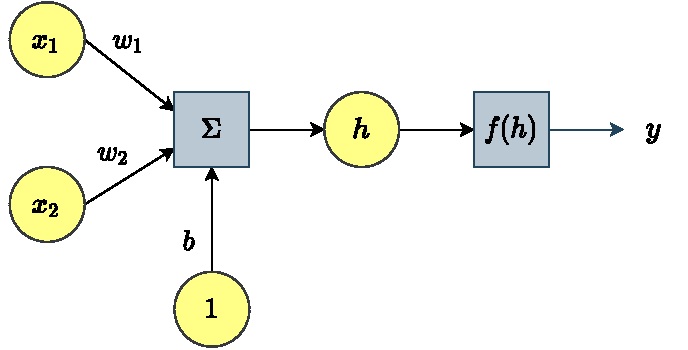
\includegraphics[height=0.6\textheight]{simple_nn}
		\caption{Diagram of a simple neural network (one perceptrón)}
		\label{fig:simple-neuron}
	\end{figure}
\end{frame}


\frame{
	\frametitle{Activation functions}
	\begin{itemize}
		\item The activation function can be any function.
	\item A nice function is the sigmoid (logistic)
	\begin{equation}
	sigmoid(x) = \dfrac{1}{1+e^{-x}}	
	\end{equation}
	\end{itemize}
\begin{center}
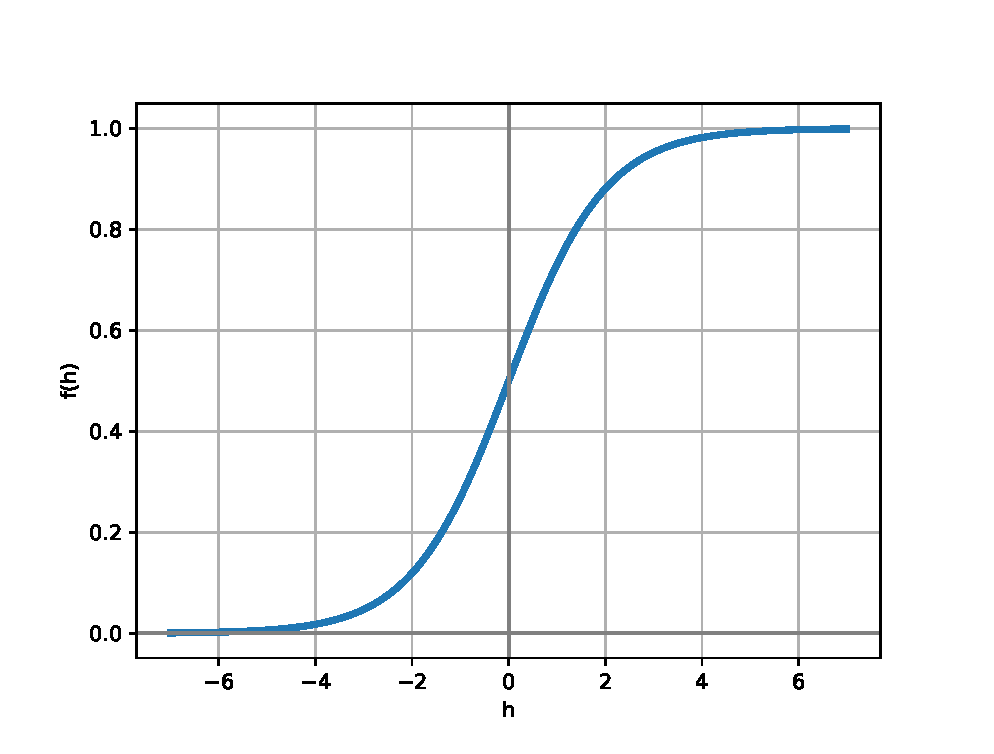
\includegraphics[height=0.6\textheight]{sigmoid_function}
\end{center}
}


\frame{
\frametitle{Activation functions}
\begin{itemize}
\item hyperbolic tangent.
\begin{equation}
	f_{tanh}(h) = \frac{e^h - e^{-h}}{e^h + e^{-h}}
\end{equation}
\end{itemize}
\begin{center}
	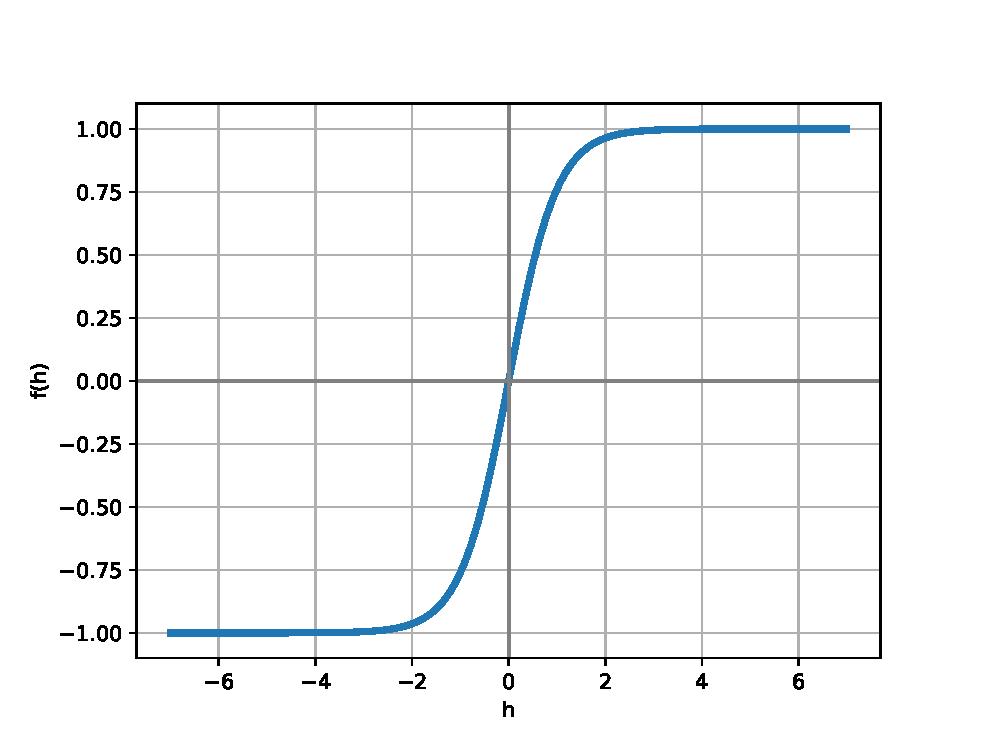
\includegraphics[height=0.6\textheight]{tanh_function}
\end{center}
}



%\frame{
%\frametitle{Excercise}
%\begin{itemize}
%	\item 02\_red\_neuronal\_simple.ipynb
%\end{itemize}
%}
		
		
\frame{
	\frametitle{The simpest NN}
	\begin{equation}
	\hat{y} = f(h) = sigmoid(\sum_{i=1}^n w_i x_i + b)
	\end{equation}
	\begin{itemize}
		\item A simple NN does not offer advantage over linear regression models.
		\item Stacking nodes provides a powerful tool versus regression models.
		\end{itemize}
}


\begin{frame}{Evolution: Rosenblatt Perceptron vs. Modern Neuron}
	\begin{block}{Key Takeaway}
		The shift to continuous activations moved Neural Networks from simple logic gates to powerful function approximators trainable via calculus.
	\end{block}
\end{frame}


\section{Weight learning}

\frame{
\frametitle{Learning}
\begin{figure}
	\centering
	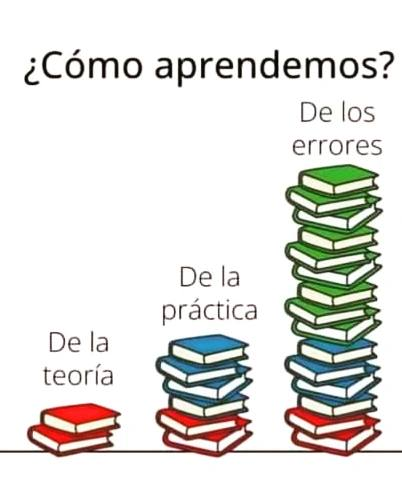
\includegraphics[height=0.70\textheight]{errores}
	\caption{Ilustración de aprendizaje. \footnote{Anderson-bastidas.com}}
	\label{fig:errores}
\end{figure}
}


%\frame{
%\frametitle{Exercise}
%	\begin{itemize}
%		\item To program the simplest NN.
%	\end{itemize}
%}


\frame{
	\frametitle{Prediction Error}
	\begin{itemize}
		\item How wrong the predictions are?
		\item Sum of squared errors (SSE)\footnote{*divided by 2 for further derivation}
		
		\begin{equation}
		E= \frac{1}{2} \sum_{\mu=1}^m \left[ y^{\mu} - \hat{y}^{\mu} \right]^2
		\end{equation} 
		where $\hat{y}$ is the prediction, $y$ is the true value and $\mu$ the data row.
	\end{itemize}
}
		
		

\frame{
	\frametitle{Learning the weights}
	\begin{itemize}
		\item Prediction 
		\begin{equation}
		\hat{y}^{\mu} = f\left( \sum_{i=1}^n w_i x^{\mu}_i + b \right)
		\end{equation}
		\item The error depends on the weights
		\begin{equation}
		E(w_i) = \frac{1}{2} \sum_{\mu=1}^m \left[ y^{\mu} - f\left( \sum_{i=1}^n w_i x^{\mu}_i + b\right)  \right]^2
		\end{equation}
		\item Our goal is to find the weights that minimice the error.
	\end{itemize}
}

%\section{Gradient descent}

\frame{
	\frametitle{Gradient Descent}
	\begin{itemize}
		\item At each step the error and the gradient are calculated, then the weights are calculated \footnote{ Rosenbloom, P. "The method of steepest descent." Proc Symp Appl Math. Vol. 6. 1956.}. 
	\end{itemize}
	
	\begin{center}
		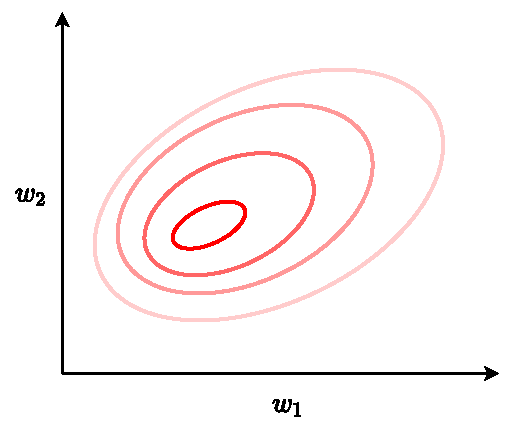
\includegraphics[height=0.6\textheight]{gradient_descent_0}
	\end{center}
}


\frame{
	\frametitle{Gradient Descent}
	\begin{itemize}
		\item At each step the error and the gradient are calculated, then the weights are calculated.
	\end{itemize}
	
	\begin{center}
		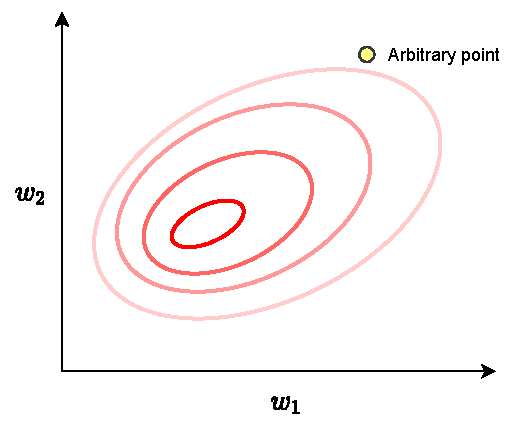
\includegraphics[height=0.6\textheight]{gradient_descent_0p}
	\end{center}
}


\frame{
	\frametitle{Gradient Descent}
	\begin{itemize}
		\item At each step the error and the gradient are calculated, then the weights are calculated.
	\end{itemize}
	
	\begin{center}
		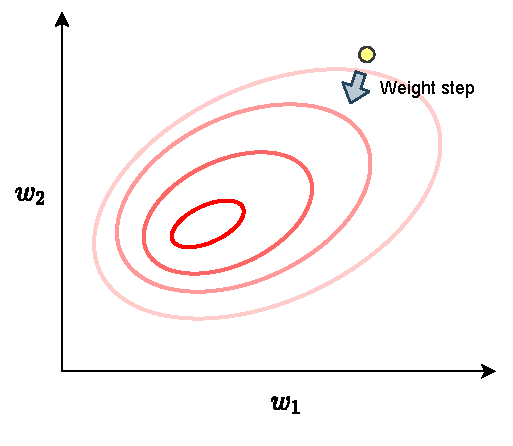
\includegraphics[height=0.6\textheight]{gradient_descent_1}
	\end{center}
}


\frame{
	\frametitle{Gradient Descent}
	\begin{itemize}
		\item At each step the error and the gradient are calculated, then the weights are calculated.
	\end{itemize}
	
	\begin{center}
		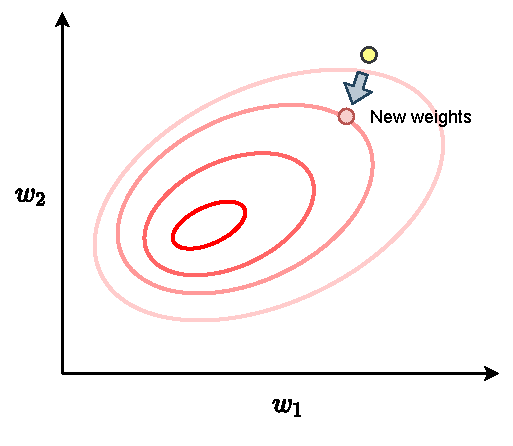
\includegraphics[height=0.6\textheight]{gradient_descent_1n}
	\end{center}
}


\frame{
	\frametitle{Gradient Descent}
	\begin{itemize}
		\item At each step the error and the gradient are calculated, then the weights are calculated.
	\end{itemize}
	
\begin{center}
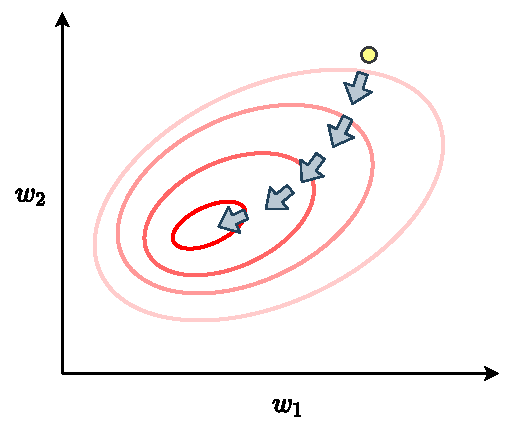
\includegraphics[height=0.6\textheight]{gradient_descent}
\end{center}
}

\frame{
	\frametitle{Gradient descent}
	\framesubtitle{Simplification Rule}
	\begin{itemize}
		\item The gradient of the error function
		\begin{equation}
			\frac{\partial E}{\partial w_i} = -(y-\hat{y})f'(h)x_i
		\end{equation}
		\item Error term
		\begin{equation}
			\delta= (y-\hat{y})f' (h) = (y-\hat{y})f' (\sum_i w_i x_i)
		\end{equation}
		\item Weight step 
		\begin{equation}
			\Delta w_i= \eta \delta x_i
		\end{equation}
		\item Weight update
		\begin{equation}
			w_i = w_i + \Delta w_i
		\end{equation}
	\end{itemize}
}

 

\frame{
	\frametitle{Activation functions}
	\begin{itemize}
		\item Derivative of the Sigmoid
		\begin{equation}
			f(x) =	sigmoid(x) = \dfrac{1}{1+e^{-x}}
		\end{equation}
		\begin{equation}
			f' = f \left( 1 - f \right) 
		\end{equation}
		\begin{figure}
			\centering
			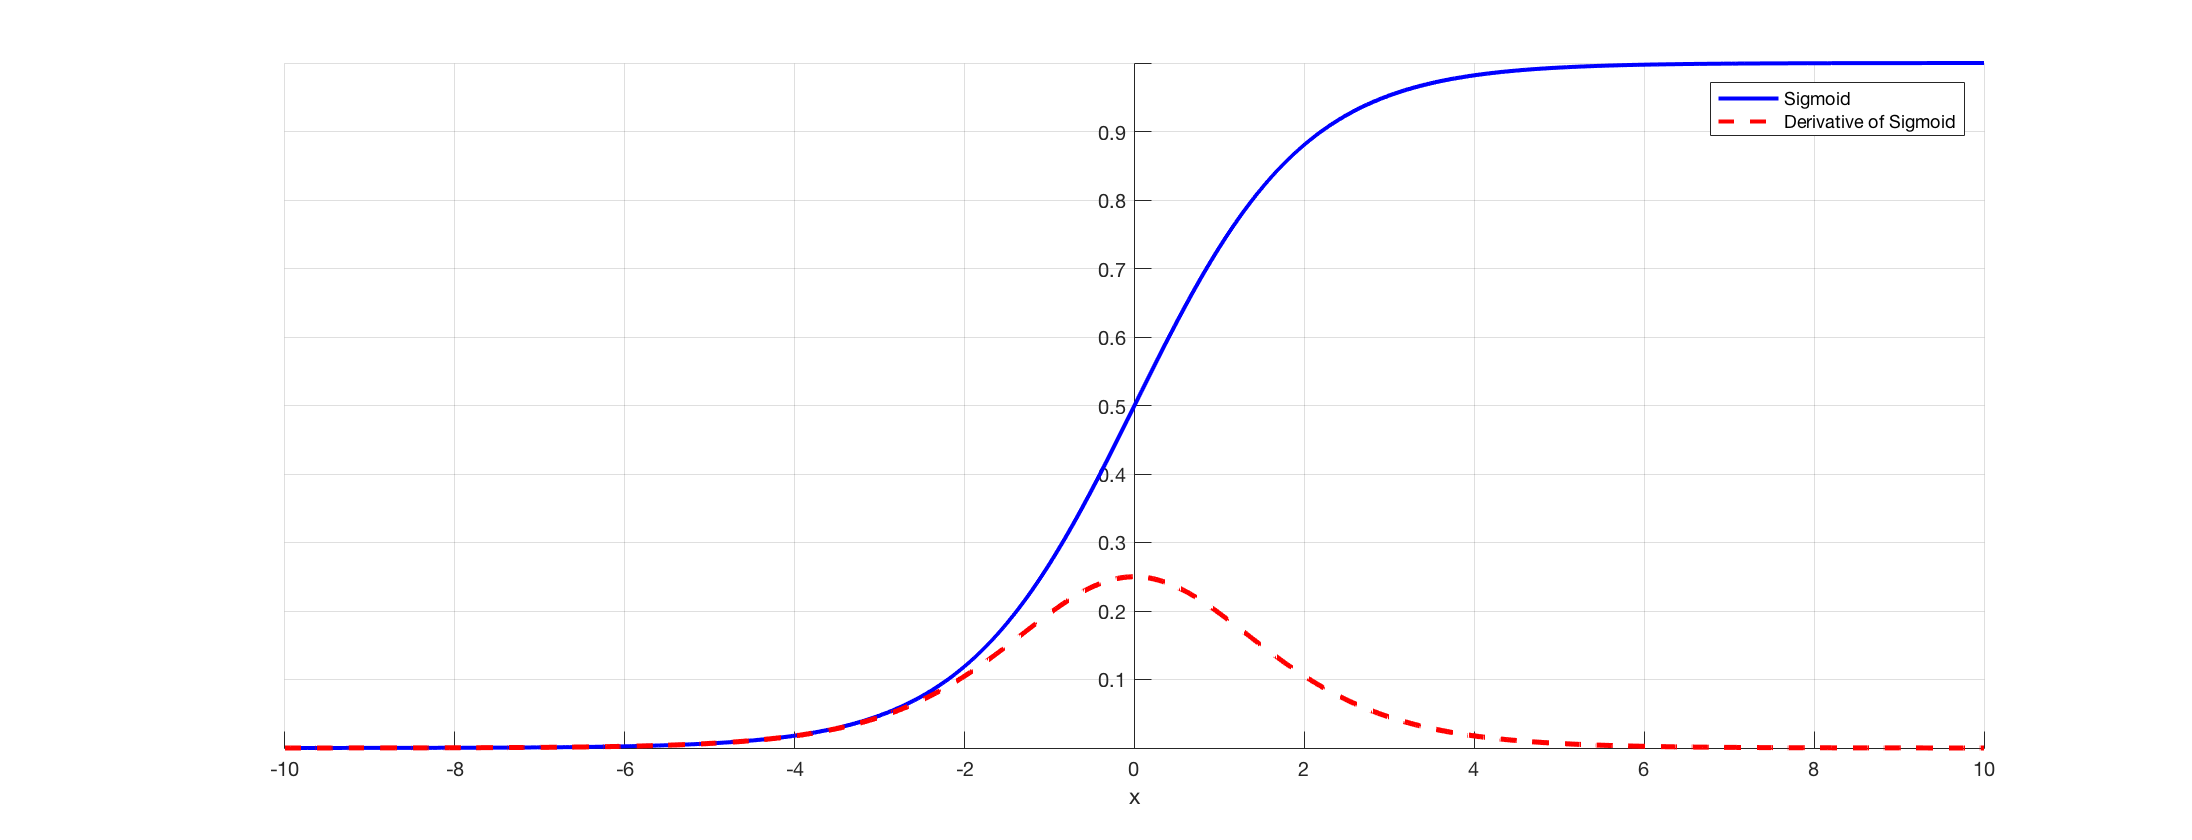
\includegraphics[height=0.5\textheight]{derivative_sigmoid}
			\caption{Sigmoid and its derivative}
			\label{fig:derivativesigmoid}
		\end{figure}
	\end{itemize}
}


\frame{
	\frametitle{Activation functions}
	\begin{itemize}
		\item Derivative of the tanh
		\begin{equation}
			\tanh(x) = \frac{e^{x} - e^{-x}}{e^{x} + e^{-x}}
		\end{equation}
		\begin{equation}
			\frac{d}{dx}\tanh(x) = 1 - \tanh^2(x)
		\end{equation}
		\begin{figure}
			\centering
			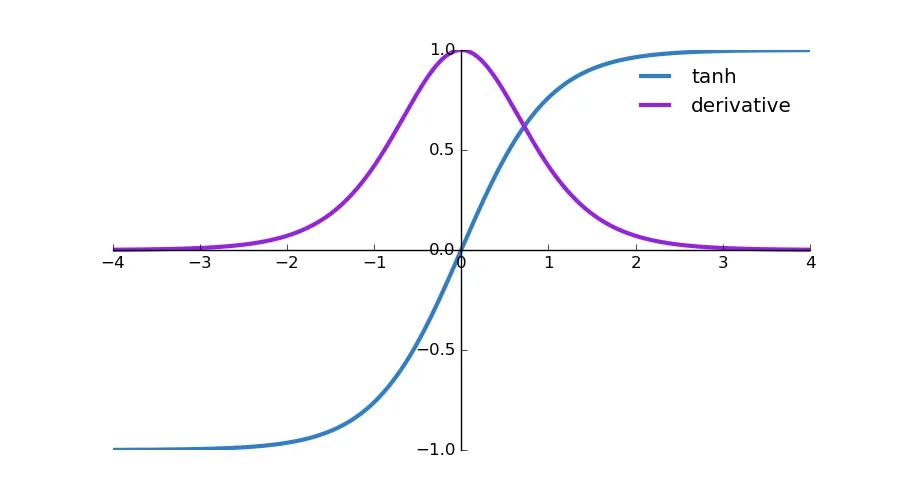
\includegraphics[height=0.5\textheight]{dtanh}
			\caption{Hiperbolic tangent and its derivative}
			\label{fig:derivativesigmoid}
		\end{figure}
	\end{itemize}
}


\frame{
	\frametitle{Gradient descent algorithm}
{\footnotesize
	\begin{algorithm}[H]
		\SetAlgoLined
		\KwData{Datos ($Data$), número de registros ($m$), tasa de aprendizaje ($\eta$), épocas ($epochs$)}
		\KwResult{Pesos entrenados ($W$)}
		%$w_i = rand(-\frac{1}{\sqrt{n}}, \frac{1}{\sqrt{n}})$ \tcc*{Inicializar pesos}
		$\texttt{Inicializar}(W)$\tcc*{Inicializar pesos}
		\For{$e=1;epochs$}{
			%\tcc{Para cada registro en la tabla de datos}
			$\text{Ceros}(\Delta W_i)$ \; 
			\ForEach{(x, y) $\in$ Data}{
				$\hat{y} = f(h(x,W))$ \tcc*{Pase frontal}
				$\delta = (y-\hat{y})f'(h)$ \tcc*{Término de error}
				\ForEach{$w_i \in W$}{
					$\Delta w_i = \Delta w_i + \delta x_i$
					\tcc*{Incremento}
				}
			}
			\ForEach{$w_i \in W$}{
				$w_i = w_i + \frac{\eta}{m} \Delta w_i $ \tcc*{Actualización normalizada}}
		}
		\KwRet{$W$}
		\caption{Descenso por gradiente}
	\end{algorithm}
 }
}


\begin{frame}
\frametitle{Neural networks}
\begin{figure}
	\centering
	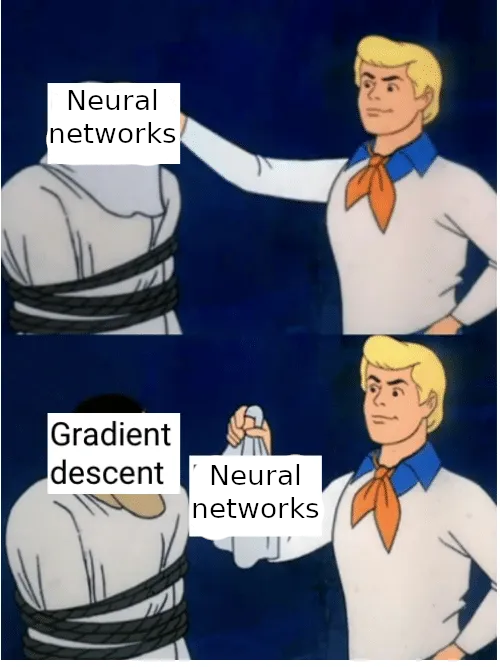
\includegraphics[height=0.8\textheight]{gdmeme}
	%\caption{Behind neural networks}
	\label{fig:gdmeme}
\end{figure}
\end{frame}


%\frame{
%	\frametitle{Exercise. Implement a simple neural network.}
%	\begin{itemize}
%		\item Given $$x = [2 , 1],$$ $$w = [-0.5,0.5],$$ $$y = 0.6,$$ $$\eta = 0.4,$$ $$f= sigmoid$$
%		\item Draw the diagram of the NN.
%		\item Calculate: i) output of the NN, ii) residual error of the NN, iii) error term and iv) weight increment,
%		%\item Help: exercise gradient descent base.py
%	\end{itemize}
%}



\section{Simple Network with multiple outputs}


\frame{
	\frametitle{Multiple outputs}
	
	\begin{figure}
		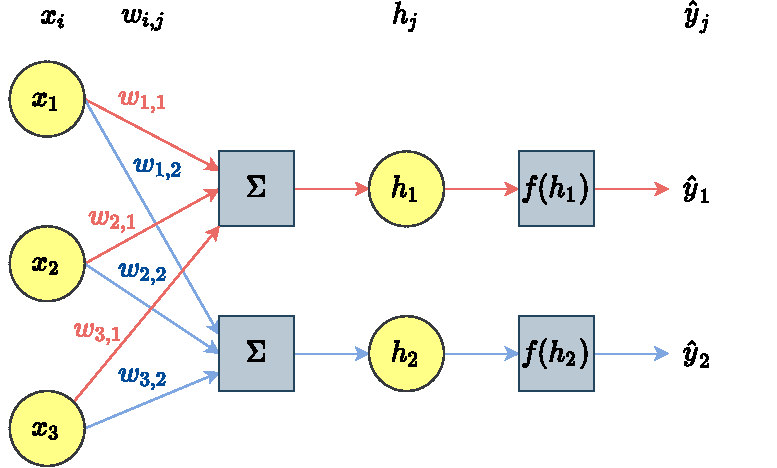
\includegraphics[height=0.6\textheight]{multiple_nn}
		\caption{Neural network with multiple outputs}
	\end{figure}
}


\frame{
	\frametitle{Learning the weights for multiple outputs}
	\begin{itemize}
		\item Prediction 
		\begin{equation}
		\hat{y}_{j}^{\mu} = f\left( \sum_i w_{i,j}
			 x_i + b \right)  
		\end{equation}
		\item Sum of squared errors (SSE)
		\begin{equation}
		E=\frac{1}{2} \sum_{\mu} \sum_j \left[ y_{j}^{\mu} - \hat{y}_{j}^{\mu} \right]^2
		\end{equation}
		where $\hat{y}$ is the prediction, $y$ is the true value, $j$ the output and $\mu$ the data row. Substituting:
		\begin{equation}
		E=\frac{1}{2} \sum_{\mu} \sum_j \left[ y_{j}^{\mu} - f\left( \sum_i w_{i,j} x_i + b\right)  \right]^2
		\end{equation}
	\end{itemize}
}



\frame{
	\frametitle{Learning the weights for multiple outputs}
	\begin{itemize}
		\item Error term 
		\begin{equation}
		\delta_j =  (y_j-\hat{y}_j)f' (h_j)
		\end{equation}
		\item Weight step
		\begin{equation}
		\Delta w_{i,j} = \eta \delta_j x_i
		\end{equation}
		\item Weight update
		\begin{equation}
		w_{i,j} = w_{i,j} + \Delta w_{i,j}
		\end{equation}
	\end{itemize}
}


\section{Practical aspects}


\frame{
	\frametitle{Mean squared error}
	\framesubtitle{Loss functions}
	\begin{itemize}
		\item Avoids the divergence from the gradient descent provoked by a large data set.
		\begin{equation}
		E = \frac{1}{m} \sum_\mu \left( y^\mu - \hat{y}^\mu \right)^2 
		\end{equation}
		\item $m$ is the number of examples
	\end{itemize}
}


\frame{
	\frametitle{Mean absolute error}
	\framesubtitle{Loss functions}
	\begin{itemize}
		\item Smaller penalization to large errors
		\begin{equation}
		E = \frac{1}{m} \sum_\mu \left|  y^\mu - \hat{y}^\mu \right|
		\end{equation}
		\item $m$ is the number of examples
	\end{itemize}
}

\begin{frame}[fragile]
\frametitle{Weights initialization}
\begin{itemize}
	\item Set bias ($b$) to zero
	\item Zero initialization for weights is not successful
	\item Random numbers is better but be careful of large numbers
\end{itemize}

\begin{figure}
	\centering
	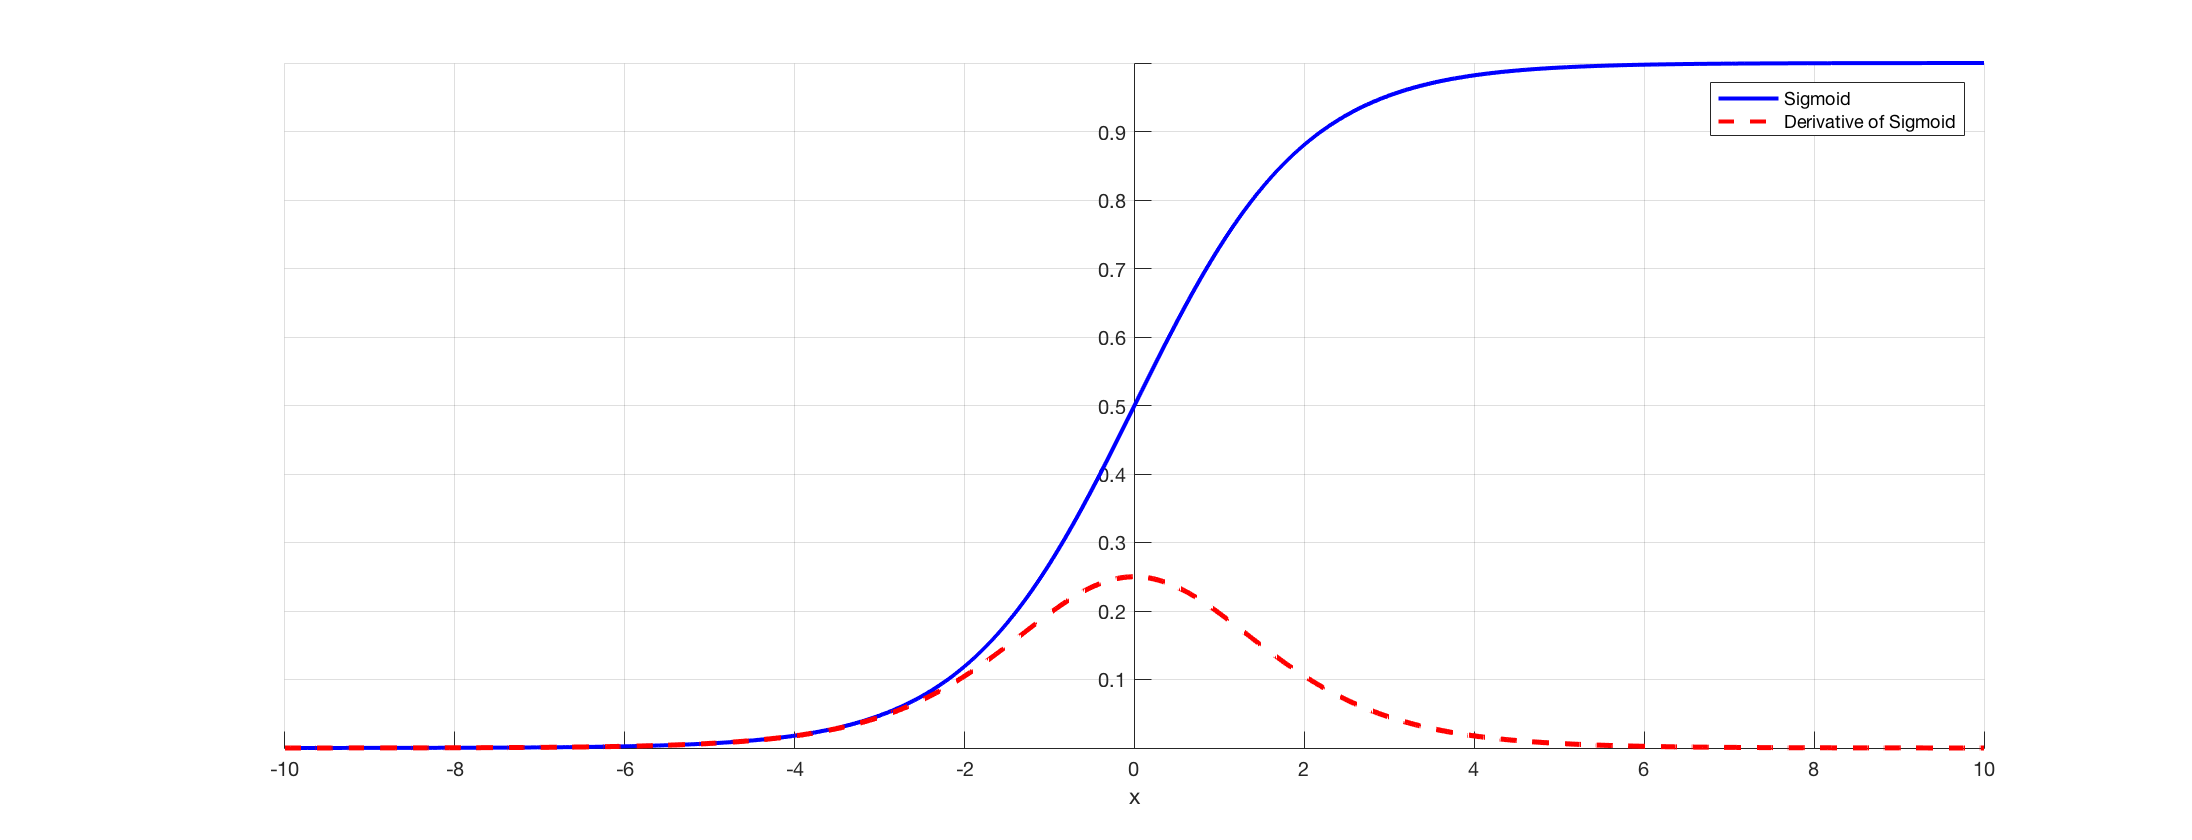
\includegraphics[height=0.5\textheight]{derivative_sigmoid}
	\caption{Sigmoid and its derivative}
	\label{fig:derivativesigmoid}
\end{figure}
\end{frame}


\begin{frame}
	\frametitle{Uniform Initialization}
	Assigns random values to the weights within a specific range.
	
	\begin{equation}
		W \sim \mathcal{U}\left( -a, a \right)
	\end{equation} where $a$ is a value that defines the boundaries of the range.
\end{frame}


\begin{frame}[fragile]
\frametitle{Weights initialization (2)}
%\begin{figure}
	\centering
	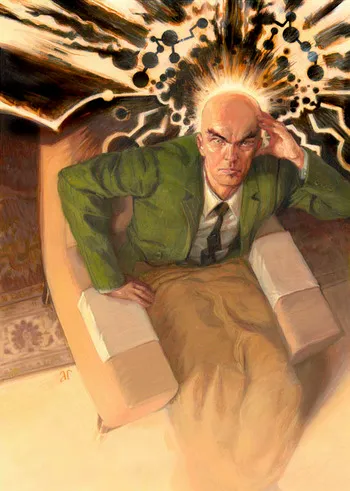
\includegraphics[height=0.45\textheight]{professor_x}
%	\caption{}
%	\label{fig:professorx}
%\end{figure}

\begin{itemize}
	\item Xavier initialization \footnote{{\scriptsize Glorot, Xavier, and Yoshua Bengio. "Understanding the difficulty of training deep feedforward neural networks." Proceedings of the thirteenth international conference on artificial intelligence and statistics. JMLR Workshop and Conference Proceedings, 2010.}}
	\begin{equation}
	W_{i,j}  \sim U(-\frac{1}{\sqrt{n}}, \frac{1}{\sqrt{n}})
	\end{equation} where $U(-a,a)$ is the uniform distribution in the interval $(-a,a)$ and $n$ is the number of input units.
\end{itemize}
\end{frame}


\begin{frame}
	\frametitle{He (Kaiming) Initialization \footnote{He, Kaiming, et al. "Delving deep into rectifiers: Surpassing human-level performance on imagenet classification." Proceedings of the IEEE international conference on computer vision. 2015.}}
	Specially designed for layers using the \textbf{ReLU} (Rectified Linear Unit) activation function or its variants.
	
	\begin{itemize}
		\item Addresses the fact that ReLU is zero for half of its domain.
		\item For a normal distribution, the weights are sampled from:
	\end{itemize}
	
	\begin{equation}
		W \sim \mathcal{N}\left( 0, \sigma^2 \right) \quad \text{where} \quad \sigma = \sqrt{\frac{2}{n_{in}}}
	\end{equation}
	
	\begin{itemize}
		\item For a uniform distribution, the range is:
	\end{itemize}
	
	\begin{equation}
		W \sim \mathcal{U}\left( -\sqrt{\frac{6}{n_{in}}}, \sqrt{\frac{6}{n_{in}}} \right)
	\end{equation}
\end{frame}



%\frame{
%	\frametitle{Multiple outputs}
	
%	\begin{center}
%		\includegraphics[width=\linewidth]{error1}
%	\end{center}
%}



\begin{frame}[fragile]
    \frametitle{Further readings}
    \begin{itemize}
		\item WIDROW, B. (1995). Perceptrons, Adalines, and Backpropagation. The Handbook of Brain Theory and Neural Networks.
	\end{itemize}
\end{frame}



%\begin{frame}[fragile]
%	\frametitle{Implementing Gradient Descent (GD)}
%	\begin{lstlisting}
%	# activation function
%	def sigmoid(x):
%	return 1/(1+np.exp(-x))
%	
%	# f prime
%	def sigmoid_prime(x):
%	return sigmoid(x) * (1 - sigmoid(x))
%	
%	# function h
%	def function_h(X, W, b):
%	return np.dot(W, X) + b
%	
%	# output of the NN
%	def function_f(X,W,b):
%	return sigmoid(function_h(X,W,b))
%	\end{lstlisting}
%\end{frame}


%\frame{
%	\frametitle{Gradient Descent Algorithm}
%	\begin{enumerate}
%		\item Set the initial weights.
%		\item Repeat for $e$ epochs.
%		\begin{enumerate}
%		\item Set the weight step to zero: $\Delta w_i = 0$
%		\item For each record in the training data:
%		\begin{enumerate}
%		   \item Make a forward pass through the network, calculating the output $\hat{y}$
%		   \item Calculate the error gradient in the output unit $\delta = (y-\hat{y})f'(h)$
%		   \item Calculate the weight step $\Delta w_i = \Delta w_i + \delta x_i$
%		\end{enumerate}
%		\item Update the weights $w_i = w_i + \frac{\eta}{m} \Delta w_i $ where $m$ is the number of records.  
%	    \end{enumerate}
%	\end{enumerate}
%}











%\frame{
%\frametitle{Exercise}
%\begin{itemize}
%\item 04 Gradient descent
%\item Draw the NN
%\item Calculate the output
%\item Calculate the error
%\item Calculate change in weights
%\item Update weights
%\end{itemize}
%}


\frame{
\frametitle{References}
 \begin{itemize}
 	\item Vasquez Gomez, Introducción a las redes neuronales, CIDETEC-IPN
 	\item Goodfellow, Ian, et al. Deep learning. Vol. 1. No. 2. Cambridge: MIT press, 2016.
 	\item Zhang, Aston, et al. Dive into deep learning. Cambridge University Press, 2023.
 	\item Stewart, James, Daniel K. Clegg, and Saleem Watson. Calculus: early transcendentals. Cengage Learning, 2020.
 	\item Buduma, Nithin, Nikhil Buduma, and Joe Papa. Fundamentals of deep learning: Designing next-generation machine intelligence algorithms. " O'Reilly Media, Inc.", 2022.
 \end{itemize}
}






%\frame{
%	\frametitle{}
%	\begin{itemize}
%		\item
%	\end{itemize}
%}

\end{document}